%************************************************
\chapter{Schedule Processing Tool}\label{ch:cifparser}
 %************************************************
 \section{Introduction}
This chapter describes techniques for working with data not currently held in a form suitable for integration, but rather held, as much rail industry data is, in various single purpose formats. Methods for constructing tools to make that transition will be discussed and examples of such tools presented, alongside a discussion of when it is appropriate to build custom tools and when third party tools are appropriate. 

While ontology based systems operate on data stored as triples, it is uncommon for rail industry data to be natively stored in this form. As such tools must be provided to convert or map this data into triple based format before it can be used with ontologies. 

In the rail industry, as with most industries, much of the data currently collected and in use resides in large relational databases. Where this is the case, R2RML tools can be used to allow access to the data in a linked format. Other data sources, however exist in a range of single purpose formats developed as needed over time. An example of a typical industry datasource, requiring conversion is timetable information. This is required by many different stake holders, thus the benefits of it being available in a linked format will be felt by a large number of different groups such as customers for journey planning, also within the rail domain it is needed for timetable planning, train identification, crew rostering, and maintenance planning amongst other tasks. The obstacles to this transition, posed by the dated and industry specific data format as well as the volume of data are representative of the challenges that will be faced moving to ontology based systems. 

These tools present answers to the question \textit{\QuestionOtherData}. The contribution these tools make to answering the question will be assessed in \autoref{sec:cifconclusions}.

\section{Transition to Linked Data}
The transition from the existing heterogeneous systems to a more integrated solution has two parts; firstly the domain must be modelled, then tools must be designed and implemented to convert the existing data to a format which can be integrated. As discussed in \autoref{ch:litreview} ontology data is considered in two parts: the \say{model}, which is known as the TBox and contains the schema information and the data itself, which is known as the ABox. 

The modelling problem is being considered by numerous other studies of which the most pertinent to this work was modelling of the broader domain as part of the work reported by \citet{Tutcher2015}.  Modelling a domain requires knowledge of both ontology modelled and the domain in question, as such it can be an obstacle to transition. This challenge continues to require skilled personnel, however as more of the domain is modelled less will need modelling when new data sources are encountered. 

\subsection{Extending the ontology}
\label{sec:addingtripples}
In order as to make new datasources available as linked data it is necessary that all the concepts represented by that datasource also be held in the ontology providing the model of the domain. Where the domain ontology lacks concepts which represent the data held, it is necessary to extend the domain ontology. When this is done, it is imperative not to recreate URIs for items already in the ontology, as such the following simple steps are taken:
 \begin{itemize}
	\item Search the Tbox for URI containing the name of the property or object under consideration;
	\item Search the Tbox for URIs with labels containing the name of the property or object under consideration;
	\item Repeat the above for any common synonyms.
\end{itemize}

As is commonly stated in the literature, if an object or property (as appropriate for the concept you wish to model) exists then human judgement needs to be used to decide whether the item found is: a URI that should be reused, a super type, or different concept to that which requires modelling. Since different modelling decisions are sometimes taken at different times, it is important to check both properties and classes for any given concept. Where a concept is not directly related to the domain and may exist in an external ontology it is considered best practice to reference the external ontology rather than redefining the concept.

Once data is modelled correctly and a tool is designed to insert the abox data in an automated fashion the model will serve as a lingua franca for making the data available to other systems that require it. Additionally it will be possible to use the data in conjunction with other data stored in ontology based systems for reasoning and the abstraction of business process to rules. For example suppose a train operating company wishes to insert an extra service, for a special event at a given time and place, which attracts spectators from many separate points of origin. By combining timetable data with a static map of the network it will be possible to work out whether it is possible to add extra services from various points of origin, given also pricing information and population density data (already available in a linked format, via DBPedia\footnote{Discussed in \autoref{sec:media}}) it would be possible to ascertain the probable profit of each such service. Note that detailed routing information (not in the files discussed in this chapter) would also be necessary in this scenario. Were the ticket barriers also integrated into such a system it would be possible to sell tickets, at a price determined to make a profit and have them only work on the correct barriers at the correct stations. All of this is possible with the existing disparate systems, but many manual integration steps are required.

\subsection{Tools for processing A-Box data}

An automated tool is required to parse the A-box data in the following circumstances:

 \begin{itemize}
 	\item The data has some value;
	\item The data is not held in a relational format; as such automated mapping tools can not be employed;
	\item The data cannot be converted using existing tools, such as OpenRefine\footnote{OpenRefine, formerly Google refine, is a very powerful open source tool which can take data in a wide variety of formats, perform simple processing and output it again in a number of formats, including RDF. More details can be found at: \url{http:\\openrefine.org/}};
	\item Manual entry is prohibitively slow due to either the volume or velocity of data received.
\end{itemize}

Where the above criteria are met a tool to process the data and add it to the ontology is required. Such a tool would perform the following steps:

 \begin{itemize}
	\item Read the data source;
	\item Convert the data source into a logical in memory representation of that data source, generally objects representing the data structure;
	\item Iterate through the in memory representation inserting each part into the data store.
\end{itemize}

Station location data is also useful in the multi-modal domain. This information is distributed alongside the schedule data and would demonstrate how position data is best modelled. Furthermore by building tools that can process and combine multiple data sources it is possible to show the benefits of using more than one data source together. 

\section{Data to be imported}

Common Infterfaces Files were selected as the source of railway data to represent in a linked format since they are representative of many formats in the rail domain that will need to be converted. Additionally since this datasource is used through out the domain its conversion will bring immediate benefits, as is demonstrated by the use of this tool and datasource as part of the demonstrator discussed in \autoref{ch:COMPASS}. 

\subsection{Legacy Resource Format}
\label{sec:datatoimport}
Currently timetables are exchanged in \say{common interface file} format, as defined in \citep{nr2007}\footnote{Available from: \url{http:\\www.atoc.org/clientfiles/files/RSPDocuments/20070801.pdf}} first issued in June 1988 and updated regularly since to reflect changes in the UK railway over that time (not least privatisation) this is a representative example of rail data. It is neither easily human readable nor as dense as a pure binary format. Rather it uses fixed length rows of 80 ASCII characters where the interpretation of a row depends on what section it is in.

The schedule file contains the following information:
\begin{itemize}
	\item Schedules
	\item Associations (where trains are split and joined for example)
	\item TIPLOC Codes - These are one of the many ways locations are refereed to within the  UK rail network.
\end{itemize}

There is also a header row at the start of the file giving a unique ID to the file and its issue date and time, along with version information and other meta-data. The file is terminated with a trailer row, to allow users to confirm they have a complete file, though no check sum or similar is employed.

The schedule rows break down further into further subtypes:
\begin{description}
	\item[Basic Schedule] This contains header information pertaining to the entire schedule, such as the type of vehicle and branding of the service.
	\item[Origin Location] The starting point of a service
	\item[Intermediate Location]  A service calling point
	\item[Changes en Route] Where anything contained in the basic schedule field changes over the course of a trains' route.
	\item[Terminating Location] The last call of the service
\end{description}
Not all record types are necessarily present for any given service.

It is possible to ascertain not just the stopping time, and place, of a given service but also some limited meta data, including two different trainIDs, which are also used by other data sources. The first ID given is the so called \say{uniqueID}\footnote{the field is defined by \citet{Hicks} as \say{The unique ID of the schedule being activated - either a letter and five numbers, or a space and five numbers for VSTP trains}. Details available at: \url{http:\\nrodwiki.rockshore.net/index.php/Train_Activation}} which is also used by certain other systems (trust train activation messages use this ID), the second ID given is the headcode. Other systems, such as train describers and signalling systems refer to the train by this code. Whilst it is guaranteed a headcode is unique on the rail network at any given point in time more than one timetabled service can have the same headcode.

\begin{minipage}{\textwidth}%I don't want this spread accross pages
\begin{lstlisting}[label={lst:cif}, caption={CIF file example}]
BSNC821721612111712030000001 POO2S178117122832000 DMUS   075      S S          P
BX         EMY                                                                  
LOGTHM    1350 13503         TB                                                 
LIGTHMNBJ           1352H00000000                                               
LIALNGEJN           1356 00000000                                               
LIALNGNJN           1356H00000000                                               
LISLEFD   1415 1416H     141514161        T                                     
LIHCKNGTN 1423 1423H     14231423         T                                     
LIHBRTBDG           1432H00000000                         2                     
LIBOSTON  1441 1445      14411445         T                                     
LISIBSEY            1452H00000000                                               
LIBELWTRJ           1459 00000000                                               
LIWAINFLT 1508H1509H     15091509         T           2                         
LTSKEGNES 1521 1524      TF                                                     

\end{lstlisting}
\end{minipage}

Each row starts with a 2 letter code to uniquely identify the type of data it holds and some row types are only valid in certain places. For example each train service definition starts with a basic schedule row, then an origin location, followed by any number (including zero) of Intermediate Location's or Changes en Route and finishing with a Terminating Location. An example is shown in \autoref{lst:cif} of a complete, but short schedule in this format. Note that the schedule starts with a `BS' or ``Basic Schedule'' line, then goes on to list calling points, with the last listed as  `TF' train finishes. The time format is twenty-four hour and the presence of an `H' after a time means ``and a half'' hence 1352H should be read as ``13:52:30''. Thirty seconds is the maximum accuracy this format allows for. 

These files can be used in conjunction with a \say{Master Station Names} file which is typically distributed at the same time. This file provides further detail about the stations refereed to in schedule. Whilst TIPLOC codes are listed in the schedule file alongside a meaningful name in English, the geographic position for example is not provided. This is included in the master station names, alongside side details of the type of services that may be connected with (bus or ferry for example) and the Routing Groups, which are used for fare calculation. By joining on the TIPLOC code it is possible to combine this data with that in the schedule file.

The size of the files to be imported also represents a significant test: the chosen schedule file was 564MB, in what has already been described as a fairly dense data format. This will result in a significantly larger amount of data if exported as turtle, which is a simple text representation of linked data, presenting challenges in terms of both processing time and available RAM. As such the system will need to be carefully optimised to fit within the memory footprint of a workstation-pc (24 GB in this case).

\section{General Software Design Patterns}
Two design patterns were considered for a system to parse schedule files: a state machine and a factory pattern. The state machine pattern, as set out by \cite{Shalyto2006}, provides loose coupling between the logic of the program and the state, which is considered through out the literature to be a key objective of any software architecture. The transition logic required for processing schedule files is very limited and thus the state machine pattern was disregarded as unnecessary in this application. The factory technique first discussed in \cite{Gamma2002} conversely is applicable to this system since it abstracts the construction of objects from the point at which they are created. This is helpful in this system since it is likely that further types of data and therefore business object will need to be added to design in the future. The system aims to be flexible as to the types of files parsed, importing both \say{Master Station Names} files and Schedules, using the same architecture. In the factory pattern \say{factory classes} are used to construct objects, rather than calling an object's constructor directly. Currently there exist two factory classes, one for each type of file processed, which build the business objects before they are inserted into the datastore. A deliberate benefit of the design is that it is easily possible to add more as required.

The graphical user interface (here on referred to as GUI) partially uses the Model View View-Model design pattern, here on referred to as MVVM, to loosen coupling with the data processing part of the application. The MVVM pattern is described by \citet{Microsoft2012} and is a common way to create GUIs when using the Windows Presentation Foundation. The Windows presentation foundation in turn is a means of creating GUI's when using the .Net framework on windows desktop machines. The MVVM pattern aims to reduce coupling between the designed user interface, which is created using only XAML and describes \emph{solely} appearance (include  interactive elements such as mouse over animations) and the way the data is formatted for presentation. In this pattern the data model is independent the view model.  Data representation and processing is removed again, thus changes to how data is presented (say from a table to a graph) have no impact on the underlying system.

\section{Software implementation} 
The schedule processing tool is designed in keeping with object orientated best practice, namely: SOLID\footnote{A good explanation of SOLID design principles, illustrated with motivational posters, may be found at \url{https:\\blogs.msdn.microsoft.com/cdndevs/2009/07/15/the-solid-principles-explained-with-motivational-posters/}} software design principles, as first set out by \citet{Martin2003}. An example of the schedule processing tool's structure and inheritance is shown in \autoref{fig:tiplocedItems}.  

 \begin{figure}[!h]
\myfloatalign
{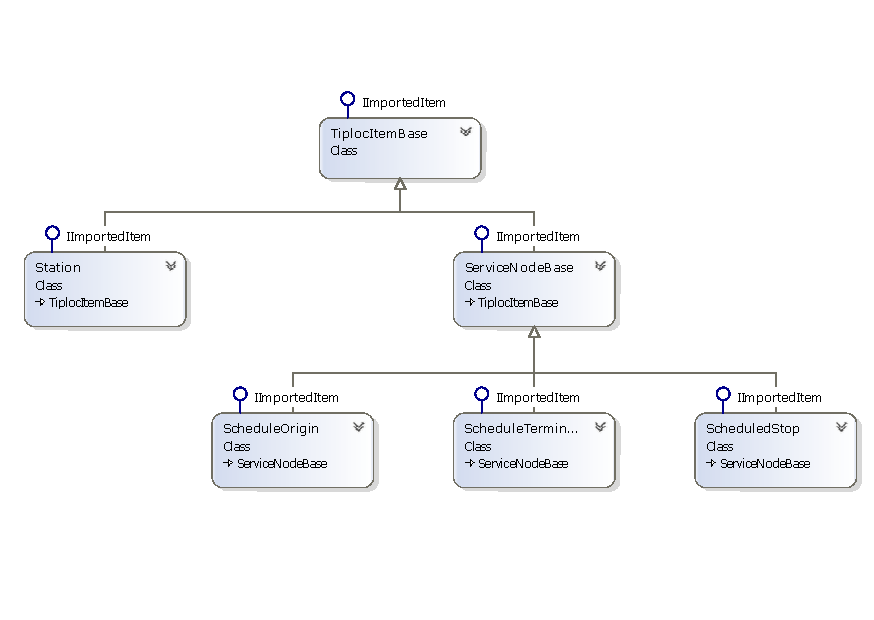
\includegraphics[width=\linewidth]{gfx/ItemsWithTIPLOCsResized}} 
\caption{Items located using a TIPLOC - one of the location codes.}
\label{fig:tiplocedItems}
\end{figure}

The business objects represent the data contained in the file, at a low level, both row by row and at slightly higher level representing schedules. All low level business objects implement the same interface, allowing for their population (from a string representing an entire line) as well as providing methods which allow for storing them to a graph. There exists a factory object for each file type parsed by the system (others can be created as needed) which handles the splitting of the source file into lines, for the creation of business objects and in particular for handling objects which are split across multiple lines, such as schedules. The business objects and the factories that create them are shown in \autoref{fig:bo}.

As a result of this design should a new file type need to be imported the tool could be extended without changes to the existing code. A framework both for reading files into memory and for inserting them into a triple stores is provided.

\begin{figure}[!h]
\myfloatalign
{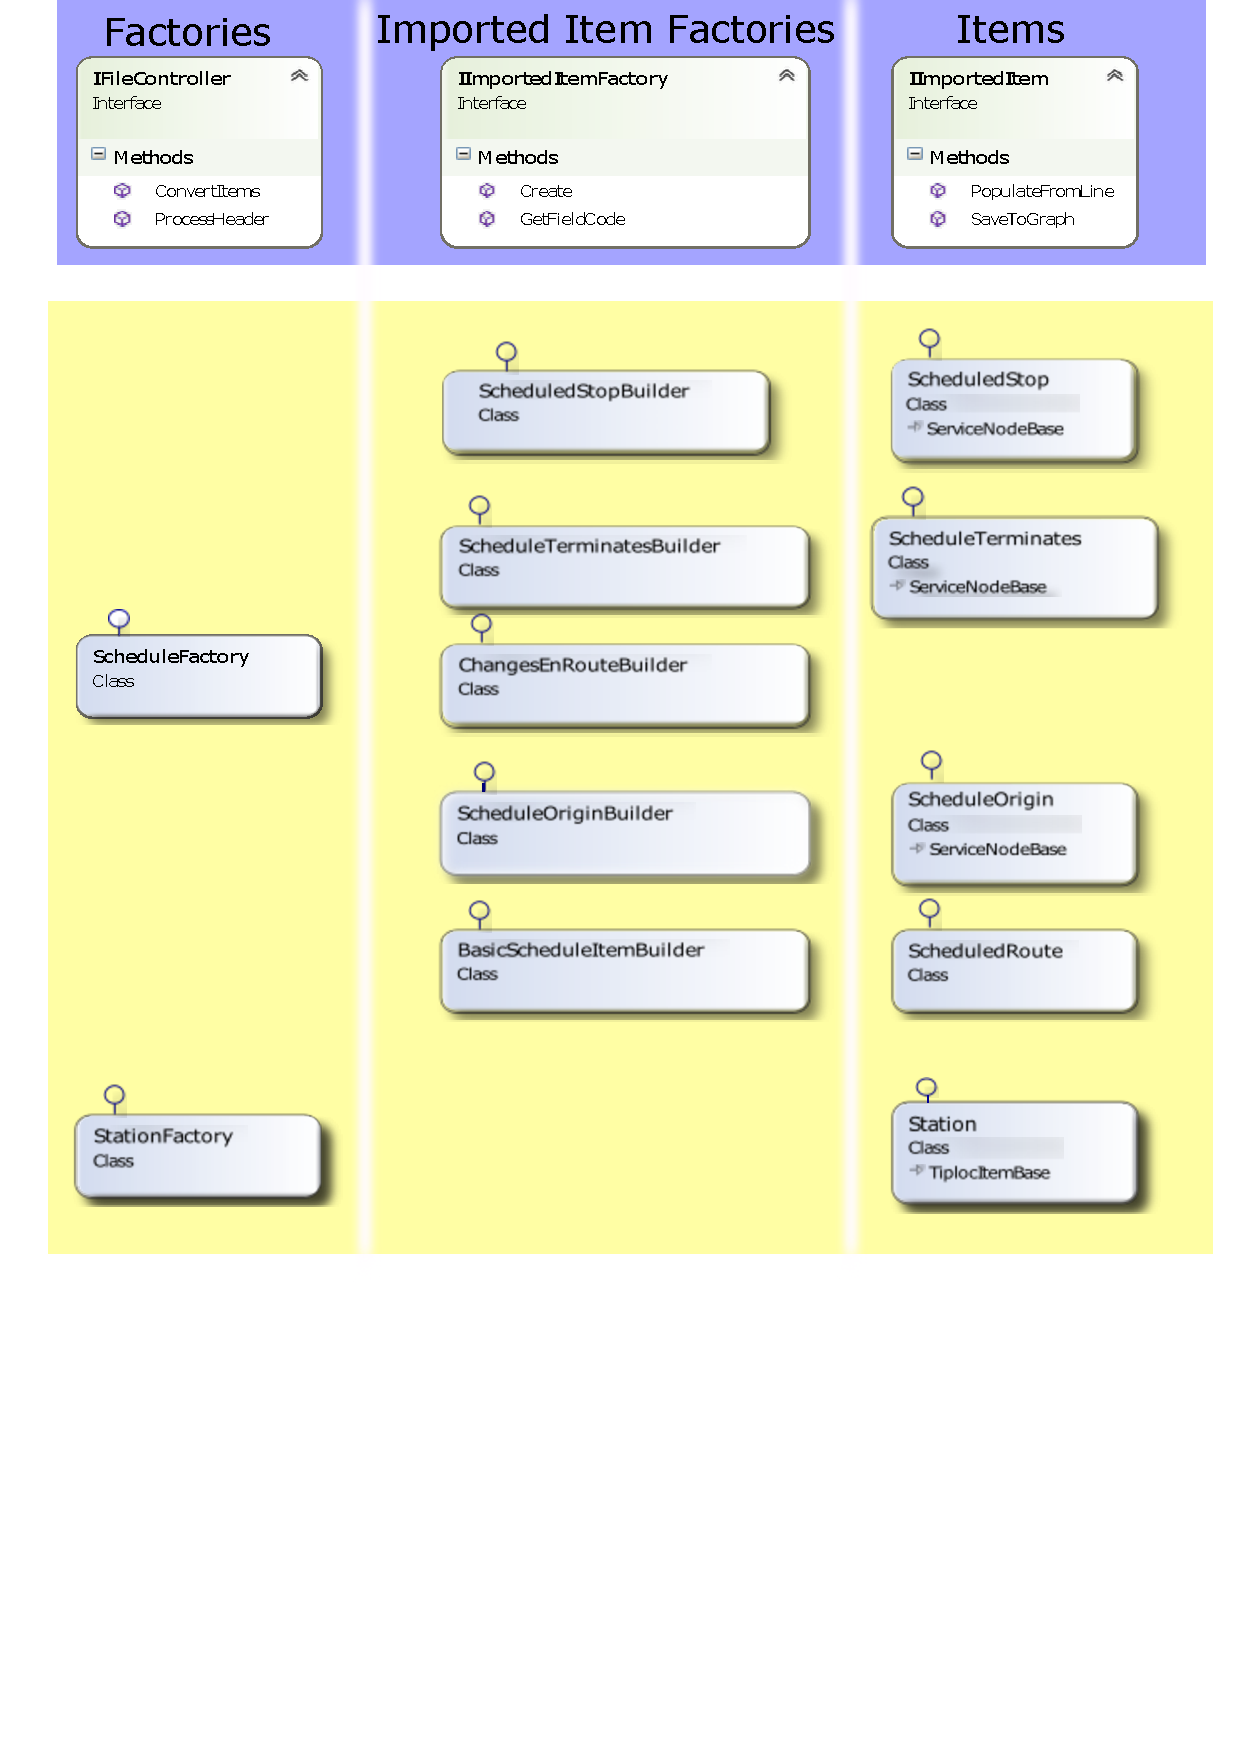
\includegraphics[width=\linewidth]{gfx/BussinessObjectsCat}} 
\caption{Business Object inheritance}
\label{fig:bo}
\end{figure}

When the business objects had been created it became apparent that some of the data they modelled was not modelled by the ontology. These fields were then added as properties in accordance with the guide lines set in \autoref{sec:addingtripples}.

Another .NET practice embraced in this project was the use of the provided settings mechanism for storing constants. This allows for changes to the settings when ever they are required as well as keeping the settings within source control and in one place for easy editing. 

An open source third party library, dotNetRD, was used for connection to local and remote triple stores. This library also allows the construction of graphs in memory and makes it possible to perform reasoning on them. This library was chosen using the fulfilled criteria:
\begin{itemize}
 \item Active maintenance;
 \item Open source (hence free to use);
 \item Compatible with the other technologies in use, in particular C\#.
\end{itemize}

It was discovered in implementing this project that when dealing with very large graphs, as was the case for schedule data, it is necessary to prevent the framework from interning all of the Uri's added as this whilst this has performance benefits they come at the cost of an enlarged memory footprint.

Given the data volumes involved it was necessary to identify bottlenecks and tasks that could be carried out in parallel and run these on separate threads. The machine used for both development and bench marking has the following pertinent specifications:
\subsection{Hardware Specification}

\noindent
\begin{tabularx}{\textwidth}{XX} 
\toprule
\textsc{Item} & \textsc{Specification}\\ 
\arrayrulecolor{LightSteelBlue}\midrule[\heavyrulewidth]
Processing & Intel i7-3820\footnote{Intel Data sheet available from: \url{http:\\ark.intel.com/products/63698/Intel-Core-i7-3820-Processor-10M-Cache-up-to-3_80-GHz}} @ 3.6 GHz. This has 4 cores and can run 8 simultaneous threads. \\
Random Access Memory & 24 Gigabytes \\
Disk & Two Terrabytes, average data rate (Read and Write) of 156 MB/s. \\
\bottomrule
\end{tabularx}
 
The graphics card fitted was of no assistance because none of the tasks in this program were suited to offload to the graphics card.

Bottlenecks were identified by running the \say{Performance Profiler} included with Visual Studio on the initial version of the software. This can tell the operator which objects are using most of the memory and which functions the schedule processing tool spends longest in. It was apparent from this that most of the memory usage was in the graph constructed by dotNetRDF and most of the processing time was in constructing that graph. In order as to achieve adequate performance, that is to be able to run an import whilst the data is still pertinent, a multi-threaded approach was required. To achieve this the data was split into chunks, after having been read from the file, but before it was materialised as a graph. Each chunk represented 500 individual elements from the underlying file, expect for the last chunk, which contained as many elements as were left. This reduced the memory footprint, since the graph was only created one chunk at a time, then stored to a file and the memory it had been occupying released. This approach also made parallel processing possible, as each chunk could be (and was) materialised separately. This design could scale linearly with the number of cores available. In order as to accomplish the multi threaded materialization and writing it was necessary to create a thread pool of data waiting to be processed and written. This uses .Net's underlying thread-pool provision but adds progress feedback and ensures that files are only written after the data is processed. The data was output as a series of turtle files, which were then inserted into a triple store using a script. This work-flow is illustrated in \autoref{fig:workflow}.

\begin{figure}[H]
\myfloatalign
\fbox{{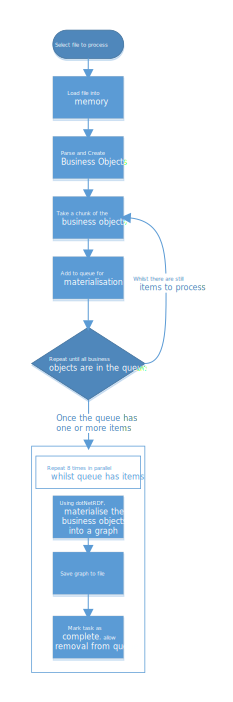
\includegraphics[max height=\textheight,max width=\linewidth]{gfx/cifParsingWorkFlow}} }
\caption{Data conversion work-flow}
\label{fig:workflow}
\end{figure}

The graphical user interface is simple and shown in \autoref{fig:cifgui}. All that was required was status feedback, for use debugging and to inform the user when the conversion was complete, and buttons to select the files to import. Also available is functionality to add provenance information to the schedules. Provenance information is added to the data when it is inserted in the ontology, allowing the source of the information to be traced, in accordance with the guide lines set out by \citet{Tutcher2015}.

\begin{figure}[H]
\myfloatalign
\fbox{{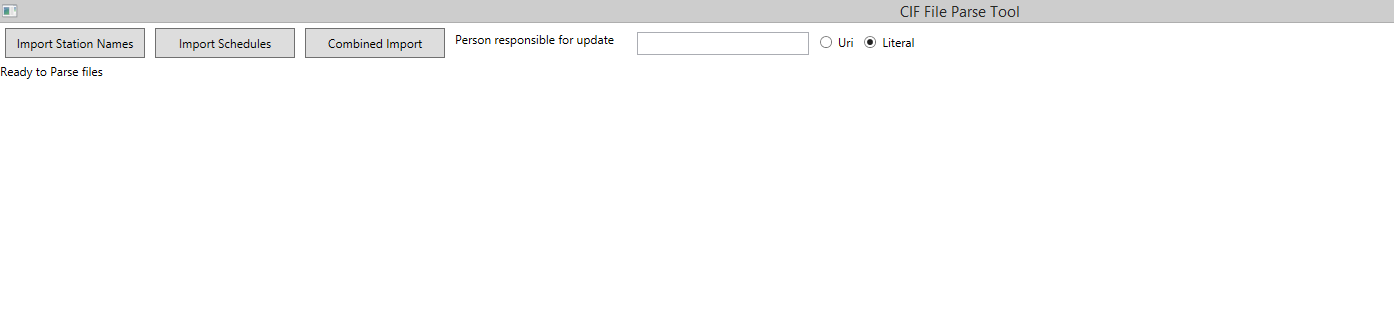
\includegraphics[max height=0.5\textheight,max width=\linewidth]{gfx/cifparseRelevantCorner}} }
\caption{Schedule parsing tool interface}
\label{fig:cifgui}
\end{figure}

\section{Manual Data Entry Tool}
\label{sec:manualtool}
The manual data entry tool demonstrates a technique for adding previously modelled low volume data to the ontologies. Where such data does not warrant the development of a bespoke tool for the task and it is not possible to interface with or alter the existing tool then a simple universal tool allowing those with no ontology engineering experience to add data to the ontology allows for improved data integration. There are many pre-existing ontology editors, both open source and commercial, of which protégé and TopBraid Composer were used during this project, however these are better suited to those with some ontology engineering experience. This tool is aimed at those with no ontology engineering experience and thus provides another possible answer to the question, \say{\QuestionOtherData}.

\subsection{Manual Data Entry Tool: Implementation}
The tool was constructed as a web application, with intent that it could be deployed centrally in large organisations and used as needed. This tool relies upon the middleware, discussed in chapter \ref{ch:middleware}, to connect to the triple store. For layout and presentation the popular \say{bootstrap}\footnote{Available from: \url{https:\\getbootstrap.com/}. This framework provides a number of styles alongside Javascript functionality} framework was employed to speed development and allow for access from a range of devices.

 \begin{figure}[H]
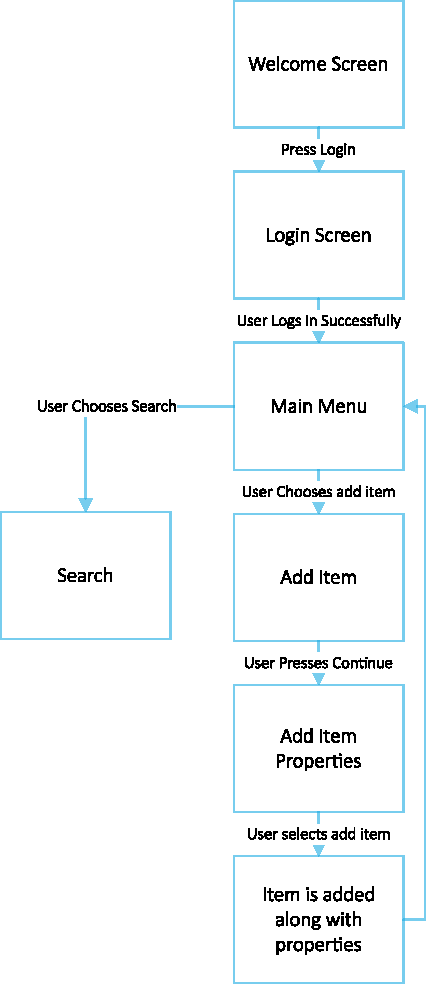
\includegraphics[max width=\linewidth]{gfx/manEntryWorkflow}
\caption{Manual Data Entry tool work flow for adding individuals to the ABox}
\label{fig:mtWorkFlow}
\end{figure}

The main menu presents user with the following options:
\begin{itemize}
    \item Adding new individuals
    \item Viewing individuals
    \item Uploading data, related to specific project, namely COMPASS as discussed in \autoref{ch:COMPASS}. 
\end{itemize}

The procedure for adding new individuals is set out in \autoref{fig:mtWorkFlow} and shown in the screenshots available in \autoref{app:mantoolgui}. In \autoref{fig:mtAddingItemDetail} (in  \autoref{app:mantoolgui}) the mechanism for supplying values for any properties that are expected is shown, the properties displayed are selected based on those that other individuals of the same class have. Users are free to enter a value or not for all of the properties shown. When done the data is then stored in the ontology.

\section{Results} 
Initial tests, on the unoptimised system, were performed with smaller schedule files, truncated to 64MB, from an original 564MB. Chunks of this size took more than twelve hours using an unoptimised version of the software, when full files were processed the program ran out of memory before returning results.

The final version of the software took two minutes and thirty four seconds to complete a cut-down (64MB input file) run. The full run took 06:46:36, which indicates that further optimisation remains possible, however this time frame would be usable.  

The files were quickly and successfully inserted into the triple store (stardog), where the inserted RDF was verified as consistent. 

As can been seen from \autoref{fig:cifparsing} in the optimised version performance is non-linear with time, as the limit of system memory is approached performance degrades significantly. A summary of the data illustrated by \autoref{fig:cifparsing} is available in \autoref{tab:cif}, which again shows that as the system consumed most of the available memory performance was significantly degraded. Through out the testing debugging tools stated that the tool alone used approximately 22 of the available 24 Gigabytes of RAM in the test system. In non-optimised versions performance was linear until all memory was consumed at which point it slowed beyond usability. The non optimised version was never run to completion, but had reached approximately 50\% completion after four days. The time spent converting this to a graph, using dotNetRDF was over five hours, where as reading the file from disk and converting it to simple, lean, business objects took twenty six seconds. 

 \begin{figure}
\myfloatalign
{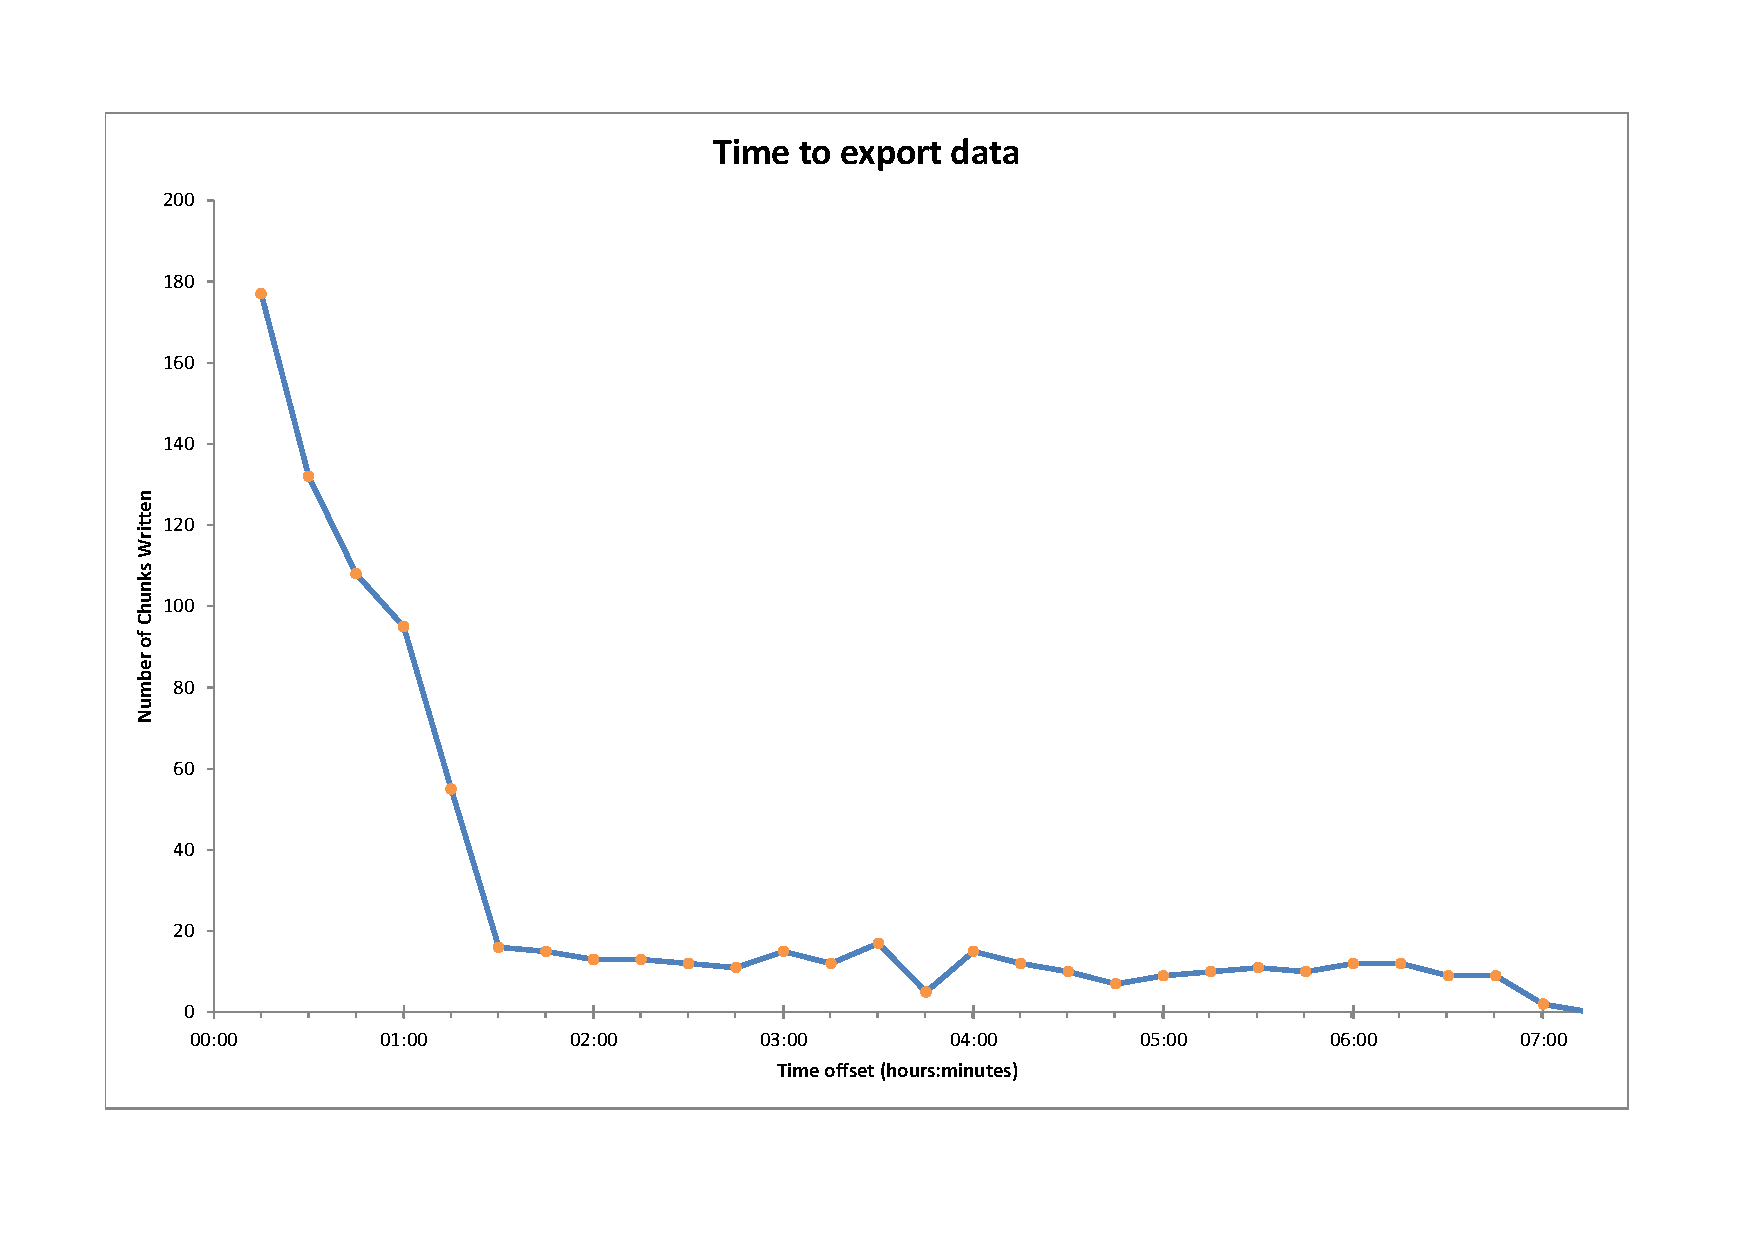
\includegraphics[width=\paperwidth]{gfx/FilesEvery15}} 
\caption{Time to output turtle files}
\label{fig:cifparsing}
\end{figure}


\noindent
\begin{table}
\begin{tabularx}{4in}{@{}cc@{}} 
\toprule \\
\textsc{Hours from Start} &  \textsc{Number of Files Produced} \\
\arrayrulecolor{LightSteelBlue}\midrule[\heavyrulewidth]
1 & 306 \\
2 & 278\\
3 & 52\\
4 & 55\\
5 & 43\\
6 & 35\\
7 & 45\\
8 & 11\\
9 & 0 (complete)\\
\bottomrule
\end{tabularx}
\caption{CIF processing times, by hour}\label{tab:cif}
\end{table}


The source code for this tool is available at: \url{https:\\github.com/Chris-MorrisUK/CifParser}.

\section{Conclusions}
\label{sec:cifconclusions}
This system was created in response to the following question: \textit{\QuestionOtherData}

Firstly this system has shown that it is possible to make typical industry data sources available in a linked format, by taking schedule data, a typical industry data source and making it available as turtle files, which can be loaded into a triple store and queried or reasoned over. 

Secondly this system has shown that even quite small data sources, as compared to video or high data rate sensors for example, require a high degree of optimisation and produce much larger data sets in a linked format. 

This design and implementation of this system also demonstrated that even where the domain has been partially modelled new applications of that model will require small alterations to suit the precise nature of the available data and its eventual use. This in turn has wide ranging implications for the need for ontology specialists to be involved, lightly at least, in the design phase of future projects making data available as an ontology.

The manual data entry tool provided another answer to the question \say{\QuestionOtherData}. For some projects the production of bespoke tools will not be financially justifiable. Where it is not possible to use commercial off the shelf software to convert data and that data is of a low enough volume then it will be possible instead to use tools to manually enter that data.

This system has also made it possible to explore: \textit{\QuestionCanOntologyScale}

The data imported covered the entire UK rail network and whilst it would have required running overnight it was none the less functional. Were the solution to be reworked so as not to create a graph of the data, then store it as turtle, but rather to directly interface with the triple store it may be possible to reduce the running time further.

\section{Further Work}
This tool could be directly connected to a datastore, thus not generating an in memory graph and serialising this to turtle files which then require insertion. This may well allow for faster processing and a smaller memory footprint. 